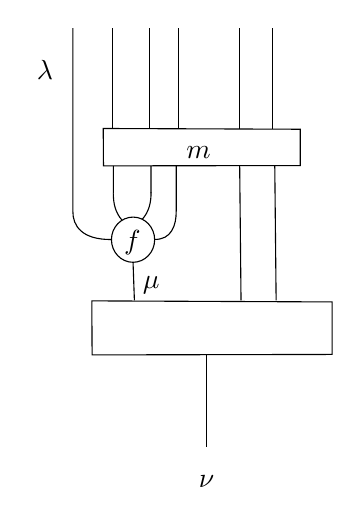
\begin{tikzpicture}[yscale=-1,scale=0.03,baseline={([yshift=-.5ex]current bounding box.center)}]
\begin{scope}[shift={(0.00mm,719.29mm)}]
% path id='path4136'
% path spec='m 348.3188,434.22405 1.19398,228.76363 1016.21342,-2.0203 0,-222.23354 z'
\draw [fill=none,draw=black] (348.32mm,434.22mm)
-- ++(1.19mm,228.76mm)
-- ++(1016.21mm,-2.02mm)
-- ++(0.00mm,-222.23mm)
-- cycle
;
% path id='path4138'
% path spec='m 974.27698,-137.78995 5.71493,570.14587'
\draw [fill=none,draw=black] (974.28mm,-137.79mm)
-- ++(5.71mm,570.15mm)
;
% path id='path4140'
% path spec='m 1122.8652,-137.91622 5.7149,570.27214'
\draw [fill=none,draw=black] (1122.87mm,-137.92mm)
-- ++(5.71mm,570.27mm)
;
% path id='path4142'
% path spec='m 522.83401,270.94502 5.76055,161.40579'
\draw [fill=none,draw=black] (522.83mm,270.95mm)
-- ++(5.76mm,161.41mm)
;
% path id='path4144'
% path spec='m 835.71429,662.36216 0,390.00014'
\draw [fill=none,draw=black] (835.71mm,662.36mm)
-- ++(0.00mm,390.00mm)
;
\node [black] at (600mm,367.02mm) { $\mu$ };
\node [black] at (834.39mm,1200mm) { $\nu$ };
\draw [fill=none,draw=black] (522.86mm,175.22mm) ellipse (91.43mm and 95.71mm) ;
% path id='path4227'
% path spec='M 476.35,92.621699 C 448.68273,61.904231 438.99734,21.774175 439.47944,-20.515368'
\draw [fill=none,draw=black] (476.35mm,92.62mm)
%%%% Warning: check controls
.. controls (448.68mm,61.90mm) and (439.00mm,21.77mm) .. (439.48mm,-20.52mm)
;
% path id='path4229'
% path spec='M 562.16133,88.454819 C 589.8286,57.737353 599.51399,17.607297 599.03189,-24.682248'
\draw [fill=none,draw=black] (562.16mm,88.45mm)
%%%% Warning: check controls
.. controls (589.83mm,57.74mm) and (599.51mm,17.61mm) .. (599.03mm,-24.68mm)
;
% path id='path4231'
% path spec='m 614.93036,174.07385 c 69.05849,0.8629 91.19261,-57.25038 90.66119,-120.460687'
\draw [fill=none,draw=black] (614.93mm,174.07mm)
.. controls ++(69.06mm,0.86mm) and ++(0.53mm,63.21mm) .. ++(90.66mm,-120.46mm)
;
% path id='path4233'
% path spec='M 431.38448,174.52373 C 306.96687,175.38538 267.08946,117.35528 268.04688,54.23544'
\draw [fill=none,draw=black] (431.38mm,174.52mm)
%%%% Warning: check controls
.. controls (306.97mm,175.39mm) and (267.09mm,117.36mm) .. (268.05mm,54.24mm)
;
% path id='path4235'
% path spec='m 267.94653,54.774248 0.0865,-774.793368'
\draw [fill=none,draw=black] (267.95mm,54.77mm)
-- ++(0.09mm,-774.79mm)
;
% path id='path4237'
% path spec='m 705.58811,54.208953 0.0869,-191.775283'
\draw [fill=none,draw=black] (705.59mm,54.21mm)
-- ++(0.09mm,-191.78mm)
;
% path id='path4239'
% path spec='m 439.40812,-19.96757 0.0868,-117.21883'
\draw [fill=none,draw=black] (439.41mm,-19.97mm)
-- ++(0.09mm,-117.22mm)
;
% path id='path4241'
% path spec='m 598.97938,-22.461088 0.0868,-114.877902'
\draw [fill=none,draw=black] (598.98mm,-22.46mm)
-- ++(0.09mm,-114.88mm)
;
% path id='path4243'
% path spec='m 396.68171,-295.5517 0.97851,158.30178 832.82908,-1.398 0,-153.78306 z'
\draw [fill=none,draw=black] (396.68mm,-295.55mm)
-- ++(0.98mm,158.30mm)
-- ++(832.83mm,-1.40mm)
-- ++(0.00mm,-153.78mm)
-- cycle
;
\node [black] at (520mm,185.44mm) { $f$ };
\node [black] at (799.84mm,-195.05mm) { $m$ };
% path id='path4257'
% path spec='m 434.36559,-295.18127 0,-424.26407'
\draw [fill=none,draw=black] (434.37mm,-295.18mm)
-- ++(0.00mm,-424.26mm)
;
% path id='path4259'
% path spec='m 594.36559,-295.18127 0,-424.26407'
\draw [fill=none,draw=black] (594.37mm,-295.18mm)
-- ++(0.00mm,-424.26mm)
;
% path id='path4261'
% path spec='m 714.36559,-295.18127 0,-424.26407'
\draw [fill=none,draw=black] (714.37mm,-295.18mm)
-- ++(0.00mm,-424.26mm)
;
% path id='path4263'
% path spec='m 974.36559,-295.18127 0,-424.26407'
\draw [fill=none,draw=black] (974.37mm,-295.18mm)
-- ++(0.00mm,-424.26mm)
;
% path id='path4265'
% path spec='m 1114.3656,-295.18127 0,-424.26407'
\draw [fill=none,draw=black] (1114.37mm,-295.18mm)
-- ++(0.00mm,-424.26mm)
;
\node [black] at (150mm,-544.78mm) { $\lambda$ };
\end{scope}
\end{tikzpicture}
